\documentclass[11pt, A4paper,norsk]{article}
\usepackage[utf8]{inputenc}
\usepackage[T1]{fontenc}
\usepackage{babel}
\usepackage{amsmath}
\usepackage{amsfonts}
\usepackage{amsthm}
\usepackage{amssymb}
\usepackage[colorlinks]{hyperref}
\usepackage{listings}
\usepackage{color}
\usepackage{hyperref}
\usepackage{graphicx}
\usepackage{cite}
\usepackage{textcomp}
\usepackage{float}

\definecolor{dkgreen}{rgb}{0,0.6,0}
\definecolor{gray}{rgb}{0.5,0.5,0.5}
\definecolor{daynineyellow}{rgb}{1.0,0.655,0.102}
\definecolor{url}{rgb}{0.1,0.1,0.4}

\lstset{frame=tb,
	language=Python,
	aboveskip=3mm,
	belowskip=3mm,
	showstringspaces=false,
	columns=flexible,
	basicstyle={\small\ttfamily},
	numbers=none,
	numberstyle=\tiny\color{gray},
	keywordstyle=\color{blue},
	commentstyle=\color{daynineyellow},
	stringstyle=\color{dkgreen},
	breaklines=true,
	breakatwhitespace=true,
	tabsize=3
}

\lstset{inputpath="C:/Users/Torstein/Documents/UiO/Fys2160/Python programmer"}
\graphicspath{{C:/Users/Torstein/Documents/UiO/Fys2160/"Python programmer"/}}
\hypersetup{colorlinks, urlcolor=url}

\author{Torstein Solheim Ølberg}
\title{Svar på Oblig nr. 1 i Fys2160}



%\lstinputlisting{Filnavn! type kodefil}
%\includegraphics[width=12.6cm,height=8cm]{Filnavn! type png}



\begin{document}
\maketitle
	\begin{center}
\Large \textbf{Oppgaver}
	\end{center}









		\paragraph{1.}
			\subparagraph{1)}
				\begin{flushleft}
I en ideel gass med en konstant temperatur er den interne energien lik den termiske energien. Da er energien gitt av loven
$$U = Nf\frac{1}{2}kT$$
Som i vårt tilfelle vil være
$$U = \frac{5}{2}NkT$$
Finner capasitansen ved å derivere
$$C_V = \frac{\partial U}{\partial T} = \frac{5}{2}Nk$$
				\end{flushleft}









			\subparagraph{2)}
				\begin{figure}[H]
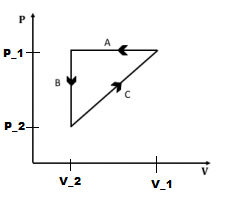
\includegraphics[width=12.6cm, height=8cm]{Figur101.png}
				\end{figure}
				\begin{flushleft}
Den interne energien $\Delta U$ er gitt ved $\Delta U = N f \frac{1}{2} k \Delta T$ der $\Delta T$ igjen er gitt ved $\Delta T = \frac{\Delta (PV)}{Nk}$. Hvis vi slår de sammen får vi at
$$\Delta U = N f \frac{1}{2} k \frac{\Delta (PV)}{Nk} = \frac{1}{2} f \Delta (PV)$$
Da blir endringen i den indre energien for de forskjellige stegene og hele syklusen
				\end{flushleft}
				\begin{gather*}
\Delta U_A = \frac{5}{2} P_1 (V_2 - V_1) \\
\Delta U_B = \frac{5}{2} (P_2 - P_1) V_2 \\
\Delta U_C = \frac{5}{2} (P_1 - P_2) (V_1 - V_2) \\
\Delta U_{tot} = \Delta U_A + \Delta U_B + \Delta U_C \\
\Delta U_{tot} = \frac{1}{2} f P_1 (V_2 - V_1) + \frac{1}{2} f (P_2 - P_1) V_2 + \frac{1}{2} f (P_1 - P_2) (V_1 - V_2) \\
\Delta U_{tot} = \frac{5}{2} \left( P_1 V_2 - P_1 V_1 + V_2 P_2 - P_1 V_2 + P_1 V_1 - P_1 V_2 - P_2 V_1 + P_2 V_2 \right) \\
\Delta U_{tot} = \frac{5}{2} \left( - P_1 V_2 - P_2 V_1 + 2 V_2 P_2 \right) \\
				\end{gather*}










			\subparagraph{3)}
				\begin{flushleft}
Arbeidet er gitt av integralet over trykket som en funksjon av volumendringen
				\end{flushleft}
				\begin{gather*}
W_A = - \int_{V_i}^{V_f} P(V) dV = - \int_{V_1}^{V_2} P_1 dV = - P_1 V_2 + P_1 V_1 = P_1 (V_1 - V_2) \\
W_B = - \int_{V_i}^{V_f} P(V) dV = 0 \\
W_C = - \int_{V_i}^{V_f} P(V) dV = - \int_{V_2}^{V_1} \frac{P_1 - P_2}{V_1 - V_2} V + P_2 dV \\
W_C = - \left[ \frac{1}{2} \frac{P_1 - P_2}{V_1 - V_2} V^2 + P_2 V \right]_{V_2}^{V_1} \\
W_C = - \left( \frac{1}{2} \frac{P_1 - P_2}{V_1 - V_2} V_1^2 - \frac{1}{2} \frac{P_1 - P_2}{V_1 - V_2} V_2^2 + P_2 V_1 - P_2 V_2 \right) \\
W_C = \frac{1}{2} \frac{P_1 - P_2}{V_1 - V_2} (V_2^2 - V_1^2) + P_2 (V_2 - V_1)  \\
W_C = \frac{1}{2} \frac{P_1 - P_2}{V_1 - V_2} (V_2 - V_1)(V_2 + V_1) + P_2 (V_2 - V_1)  \\
W_C = - \frac{1}{2} (P_1 - P_2)(V_2 + V_1) - P_2 (V_1 - V_2)  \\
\text{Dette virker rart, burde fått arealet mellom linja $C$ og $x$-aksen, ville jeg trodd} \\
W_{\text{tot}} = \oint_{ABC} P(V) = W_A + W_B + W_C \\
W_{\text{tot}} = P_1 (V_1 - V_2) - \frac{1}{2} (P_1 - P_2)(V_2 + V_1) - P_2 (V_1 - V_2) \\
W_{\text{tot}} = (P_1 - P_2) \left( (V_1 - V_2) - \frac{1}{2} (V_1 + V_2) \right)
				\end{gather*}
			









			\subparagraph{4)}
				\begin{flushleft}
Varmeutvekslingen er gitt ved
$$\Delta U = Q + W \Rightarrow Q = \Delta U - W$$
				\end{flushleft}
				\begin{gather*}
Q_A = \Delta U_A - W_A = \frac{5}{2} P_1 (V_2 - V_1) - P_1 (V_1 - V_2) \\
Q_A = \frac{7}{2} P_1 (V_2 - V_1) \\
Q_B = \Delta U_B - W_B = \Delta U_B = \frac{5}{2} (P_2 - P_1) V_2 \\
Q_C = \Delta U_C - W_C = \frac{5}{2} (P_1 - P_2) (V_1 - V_2) - \frac{1}{2} (P_1 - P_2)(V_2 + V_1) - P_2 (V_1 - V_2) \\
Q_C = \frac{1}{2} \left( (P_1 - P_2) \left( (V_1 - V_2) \left( 5 - P_2 \right) - (V_2 + V_1) \right) \right) \\
Q_{\text{tot}} = Q_A + Q_B + Q_C \\
Q_{\text{tot}} = \frac{7}{2} P_1 (V_2 - V_1) + \frac{5}{2} (P_2 - P_1) V_2 + \frac{1}{2} ( ( P_1 - P_2 ) ( ( V_1 - V_2 ) ( 5 - P_2 ) - ( V_2 + V_1 ) ) ) \\
Q_{\text{tot}} = \frac{1}{2} \left( 7 P_1 (V_2 - V_1) + 5 (P_2 - P_1) V_2 + ( P_1 - P_2 ) ( ( V_1 - V_2 ) ( 5 - P_2 ) - ( V_2 + V_1 ) ) \right)
				\end{gather*}









			\subparagraph{5)}
				\begin{flushleft}
$\Delta U$ for hele syklusen har fortegnet minus på grunn av at de tre leddene i uttrykket for endringen er henholdsvis negativ, negativ og positiv. Dette er jo da ikke egentlig en sikkerhet for at den fullstendige endringen er negativ, men siden det positive leddet bare er ett og det er et produkt av to mindre verdier, er dette det mest sannsynlige. \\
Når det kommer til $W$ for hele syklusen så er det to ledd, der det første er positivt og det andre er negativt, men delt på to. Det betyr at produktet, og dermed $W$, antageligvis er positivt. \\
For varmen $Q$ for hele syklusen er det 4 ledd, der det første er negativt, det andre er negativt, det tredje er kanskje positivt, avhengig av $P_2$ og det fjerde er negativt. Siden de tre negative leddene virker størst og alle kan være negative tipper jeg denne er det også. \\
I steg A så synker volumet samtidig som trykket holdes likt. Da virker det som at gassen blir komprimert samtidig som noe av den unnslipper kammeret. Deretter i B er det bare ekspandering av gassen, siden trykket synker, men volumet holdes likt. Det kan også komme av at gassen overfører termisk energi til omgivelsene. Så, til slutt, i C ser det ut som at det blir påført mer gass siden både volumet og trykket øker, eventuelt at det blir tilført termisk energi til gassen som også vil gjøre at tryk og volum øker.
Når volumet til gassen øker vil antageligvis gassen gjøre et arbeid på stempelet.
				\end{flushleft}









		\paragraph{2.}
			\subparagraph{1)}
				\begin{flushleft}
I et system med $N$ uavhengige spinn, som kan være opp eller ned, så er det $2^N$ forskjellige mikrotilstander.
				\end{flushleft}









			\subparagraph{2)}
				\begin{flushleft}
Hvis jeg antar at jeg kjenner til mengden med positive spinn, og totalt antall spinn $N$ så blir uttrykket
$$S = N_+ - (N - N_+) = 2N_+ - N$$
				\end{flushleft}












			\subparagraph{3)}
				\begin{figure}
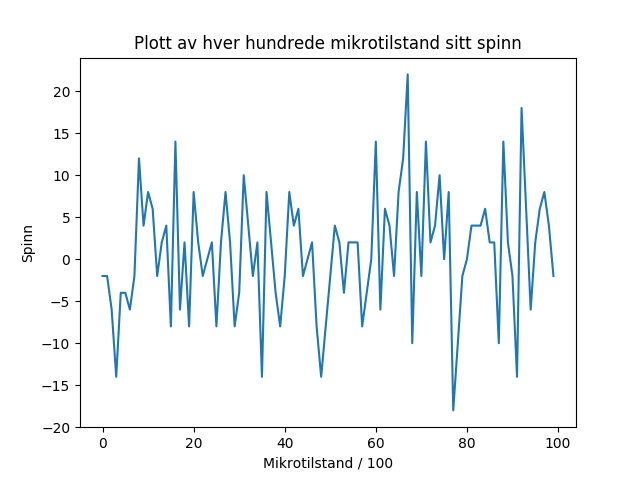
\includegraphics[width=12.6cm, height=8cm]{Figur102.png}
\caption{Plott av spinnene i oppgave 2.3}
				\end{figure}
				\begin{figure}
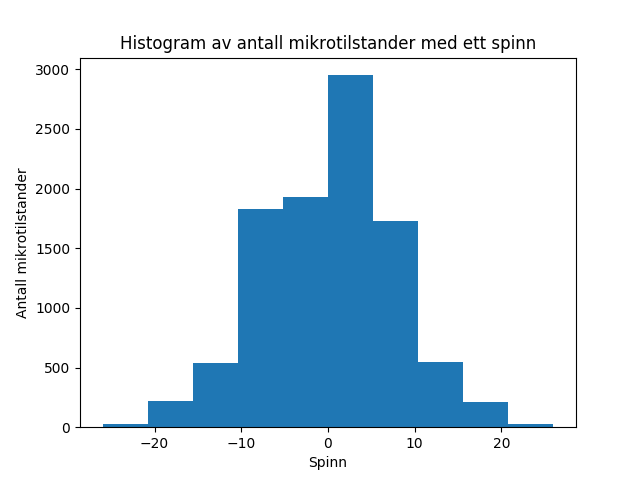
\includegraphics[width=12.6cm, height=8cm]{Figur103.png}
\caption{Histogrammet av net spinn i oppgave 2.3}
				\end{figure}
\lstinputlisting{Oblig1_2_3.py}
				\begin{flushleft}
Histogramet er enkelt å se at er ganske gaussiske fordelt, med en topp rundt null og et avvik på rundt $30$
				\end{flushleft}














			\subparagraph{4)}
				\begin{gather*}
\Omega(N, n) = \frac{N!}{n! \cdot (N - n)!} \\
n_{\text{opp}} = \text{antall spinn opp} \\
n_{\text{ned}} = \text{antall spinn ned} \\
S = \text{netto spinn} = n_{\text{opp}} - n_{\text{ned}} \\
N = \text{total antall spinn} = n_{\text{opp}} + n_{\text{ned}} \\
n_{\text{ned}} = N - n_{\text{opp}} \\
S = n_{\text{opp}} + n_{\text{opp}} - N \\
n_{\text{opp}} = \frac{S + N}{2} \\
\text{Setter inn uttrykket for $n_{\text{opp}}$ i multiplisitetsuttrykket og får} \\ 
\text{en funksjon av $N$ og $S$} \\
\Omega(N, S) = \frac{N!}{\left( \frac{S + N}{2} \right)! \left( N - \frac{S + N}{2} \right)!} = \frac{N!}{\left( \frac{S + N}{2} \right)! \left( \frac{N - S}{2} \right)!}
				\end{gather*}









			\subparagraph{5)}
				\begin{gather*}
\Omega (N, S) = \frac{N!}{\left( \frac{S + N}{2} \right)! \left( \frac{N - S}{2} \right)!} \\
\ln(a!) = a \ln(a) - a \\
\ln (\Omega) = \ln(N!) - \left( \ln \left( \frac{N + S}{2} ! \right) + \ln \left( \frac{N - S}{2} ! \right) \right) \\
\ln (\Omega) = N \ln(N) - N - \left( \frac{N + S}{2} \right) \ln \left( \frac{N + S}{2} \right) + \left( \frac{N + S}{2} \right) \\
- \left( \frac{N - S}{2} \right) \ln \left( \frac{N - S}{2} \right) + \left( \frac{N - S}{2} \right) \\
\ln (\Omega) = N \ln(N) - \left( \frac{N + S}{2} \right) \ln \left( \frac{N + S}{2} \right) - \left( \frac{N - S}{2} \right) \ln \left( \frac{N - S}{2} \right) \\
\ln (\Omega) = N \ln(N) - \left( \frac{N + S}{2} \right) ( \ln ( N + S ) - \ln(2) ) - \left( \frac{N - S}{2} \right) ( \ln ( N - S ) - \ln(2) ) \\
\ln (\Omega) = \frac{1}{2} \left( 2 N \ln(N) - ( N + S ) ( \ln ( N + S ) - \ln(2) ) - ( N - S ) ( \ln ( N - S ) - \ln(2) ) \right)
				\end{gather*}
				\begin{gather*}
\text{Prøver en ny versjon av Sterlings} \\
\Omega (N, S) = \frac{N!}{\left( \frac{S + N}{2} \right)! \left( \frac{N - S}{2} \right)!} \\
a! = a^a e^{-a} \\
\Omega = \frac{N^N e^{-N}}{\left( \frac{S + N}{2} \right)^{\left( \frac{S + N}{2} \right)} e^{- \left( \frac{S + N}{2} \right)} \left( \frac{N - S}{2} \right)^{\left( \frac{N - S}{2} \right)} e^{-\left( \frac{N - S}{2} \right)}} \\
\Omega = \frac{ N^N e^{- N + \left( \frac{S + N}{2} \right) + \left( \frac{N - S}{2} \right)} }{ \left( \frac{S + N}{2} \right)^{\left( \frac{S + N}{2} \right)} \left( \frac{N - S}{2} \right)^{\left( \frac{N - S}{2} \right)} } \\
\Omega = \frac{ N^N }{ \left( \frac{S + N}{2} \right)^{\left( \frac{S + N}{2} \right)} \left( \frac{N - S}{2} \right)^{\left( \frac{N - S}{2} \right)} }
				\end{gather*}
				\begin{flushleft}
Jeg finner ikke fem til formelen jeg skal finne ved hjelp av det jeg har gjort her. Men denne formelen er gyldig når $N \gg 1$, og hvis du bare er ute etter riktig størrelsesordenen.
Maximumet til multiplisiteten til en paramagnet for stor $N$ er gitt ved å regne ut multiplisiteten til tilstanden der $N_{\text{opp}}$ og $N_{\text{ned}}$ er like og lik $\frac{N}{2}$.
				\end{flushleft}
				\begin{gather*}
\Omega(N, N_{\text{opp}}, N_{\text{ned}}) = \frac{N!}{N_{\text{opp}}! N_{\text{ned}}!} \\
\Omega_{\text{max}} = \frac{N!}{\frac{N}{2}!^2} \\
\text{Bruker Sterlings aproksimasjon, $a! = a^a e^{-a}\sqrt{2 \pi a}$} \\
\Omega_{\text{max}} = \frac{N^N e^{-N}\sqrt{2 \pi N}}{\left( \left( \frac{N}{2} \right)^{\frac{N}{2}} e^{-\frac{N}{2}} \sqrt{2 \pi \frac{N}{2}} \right)^2} = \frac{N^N e^{-N}\sqrt{2 \pi N}}{\left( \frac{N}{2} \right)^{N} e^{-N} 2 \pi \frac{N}{2}} = 2^{N} \sqrt{\frac{2}{\pi N}}
				\end{gather*}











			\subparagraph{6)}
				\begin{figure}[H]
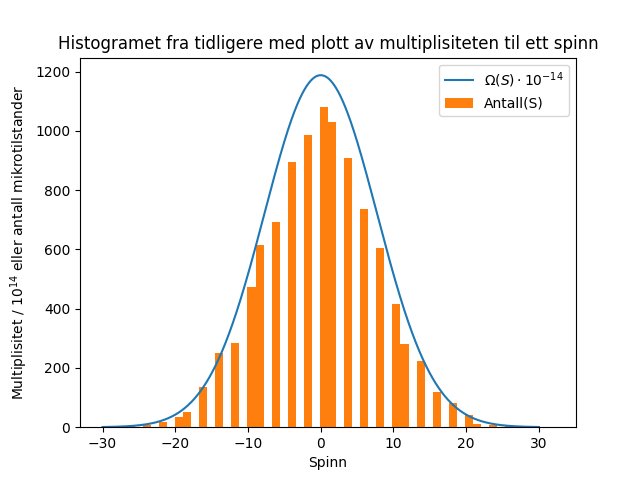
\includegraphics[width=12.6cm,height=8cm]{Figur104.png}
\caption{Plott av histogram, fra tidligere bare litt mer søyler og ett nytt sett med tilfeldige tall, og plott av den analytiske funksjonen for multiplisitet.}
				\end{figure}
				\begin{flushleft}
Ser at de til "funksjonene" begge viser en gaussisk fordeling, men at den analytiske funksjonen måtte skaleres ned med en faktor $10^{-14}$ for at de skulle kunne plottes sammen.
				\end{flushleft}
\lstinputlisting{Oblig1_2_6.py}











			\subparagraph{7)}
				\begin{flushleft}
Setter funksjonen for multiplisiteten fra forrige oppgave inn i Boltzmanns formel for entropien og får uttrykket
$$S_B = k \ln\left( 2^{N} \sqrt{\frac{2}{\pi N}} e^{\frac{- S^2}{2N}} \right) = k \left( N \ln(2) + \frac{1}{2} \ln \left( \frac{2}{\pi N} \right) - \frac{S^2}{2N} \right)$$
				\end{flushleft}
				\begin{figure}[H]
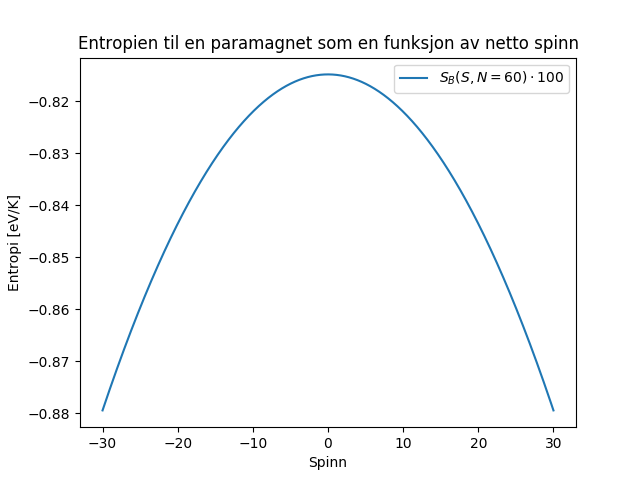
\includegraphics[width=12.6cm,height=8cm]{Figur105.png}
\caption{Plott av entropien i oppgave $2.7$}
				\end{figure}
\lstinputlisting{Oblig1_2_7.py}
\end{document}